% Use only LaTeX2e, calling the article.cls class and 12-point type.

\documentclass[12pt]{article}

% Users of the {thebibliography} environment or BibTeX should use the
% scicite.sty package, downloadable from *Science* at
% http://www.sciencemag.org/authors/preparing-manuscripts-using-latex 
% This package should properly format in-text
% reference calls and reference-list numbers.

\usepackage{scicite}

\usepackage{times}

% The preamble here sets up a lot of new/revised commands and
% environments.  It's annoying, but please do *not* try to strip these
% out into a separate .sty file (which could lead to the loss of some
% information when we convert the file to other formats).  Instead, keep
% them in the preamble of your main LaTeX source file.


%%%%%% taken from papaja-created ver
\usepackage{csquotes}
\usepackage{graphicx}
  \usepackage[unicode=true]{hyperref}
  
% The following parameters seem to provide a reasonable page setup.

\topmargin 0.0cm
\oddsidemargin 0.2cm
\textwidth 16cm 
\textheight 21cm
\footskip 1.0cm


%The next command sets up an environment for the abstract to your paper.

\newenvironment{sciabstract}{%
\begin{quote} \bf}
{\end{quote}}


%EY: to add S to figure number in supplementary materials
\newcommand{\beginsupplement}{%
        \setcounter{table}{0}
        \renewcommand{\thetable}{S\arabic{table}}%
        \setcounter{figure}{0}
        \renewcommand{\thefigure}{S\arabic{figure}}%
     }


% Include your paper's title here

\title{Polite speech arises from desires to be helpful and look helpful} 


% Place the author information here.  Please hand-code the contact
% information and notecalls; do *not* use \footnote commands.  Let the
% author contact information appear immediately below the author names
% as shown.  We would also prefer that you don't change the type-size
% settings shown here.

\author
%{Erica J. Yoon,$^{1\ast}$ Michael Henry Tessler,$^{1\ast}$ Noah D. Goodman,$^{1}$ Michael C. Frank$^{1}$\\
%\\
%\normalsize{$^{1}$Department of Psychology, Stanford University}\\
%\\
%\normalsize{$^\ast$These authors contributed equally to this work.}
%
%}
{Erica J. Yoon,$^{1\ast\dagger}$ Michael Henry Tessler,$^{1\ast}$ Noah D. Goodman,$^{1}$ Michael C. Frank$^{1}$\\
\\
\normalsize{$^{1}$Department of Psychology, Stanford University,}\\
\normalsize{450 Serra Mall, Stanford, CA 94305.}
\\
\normalsize{$^\ast$These authors contributed equally to this work.}
\\
\normalsize{$^\dagger$To whom correspondence should be addressed; E-mail: ejyoon@stanford.edu.}
}

% Include the date command, but leave its argument blank.

\date{}



%%%%%%%%%%%%%%%%% END OF PREAMBLE %%%%%%%%%%%%%%%%



\begin{document} 

% Double-space the manuscript.

\baselineskip24pt

% Make the title.

\maketitle 



% Place your abstract within the special {sciabstract} environment.

%\begin{sciabstract}
%Conveying information in a false or indirect manner in consideration of
%listeners' wants (i.e.~being polite) seemingly contradicts an important
%goal of communication: information transfer. We model production
%of polite speech in which speakers deviate from being maximally
%informative for social reasons. We show that speakers produce polite
%speech due to their desires to be helpful -- both epistemically (convey
%the true state to the listener) and socially (make the listener feel
%good) -- and to \emph{appear} helpful. We formalize this tradeoff
%between speaker's goals within a probabilistic model and show the model
%is able to predict people's polite speech production judgments. Our
%extension of formal language modeling frameworktheories of language to account for speakers' social
%goals represents an advance in understanding of human speech.
%\end{sciabstract}


\begin{sciabstract}
People often deviate from saying the maximally informative and succinct message 
(e.g.~\enquote{Your talk was terrible}) 
and instead speak \emph{politely}: 
Speakers convey information in a false or indirect manner in consideration of listeners' wants
(e.g.~\enquote{It was a great talk!}; \enquote{The talk wasn't bad; it's hard to give a good presentation anyway}). 
If language is an important means of information transfer, does polite speech contradict cooperative communication?
We argue that polite speech reflects a cooperative speaker's desire to balance between two communicative goals: 
to be \emph{epistemically} helpful and convey the true state to the listener;
and to be \emph{socially} helpful and make the listener feel good.
We also argue that a polite speaker has a desire to \emph{look} helpful and 
appear to have these two goals in mind. 
We formalize the tradeoff between the speaker's goals within a probabilistic model 
and show the model is able to predict people's polite speech production judgments. 
Our extension of formal theories of communication to account for speakers' social
goals represents an advance in understanding of human speech.
\end{sciabstract}



% In setting up this template for *Science* papers, we've used both
% the \section* command and the \paragraph* command for topical
% divisions.  Which you use will of course depend on the type of paper
% you're writing.  Review Articles tend to have displayed headings, for
% which \section* is more appropriate; Research Articles, when they have
% formal topical divisions at all, tend to signal them with bold text
% that runs into the paragraph, for which \paragraph* is the right
% choice.  Either way, use the asterisk (*) modifier, as shown, to
% suppress numbering.

Human speech is an important means of exchanging information, but
intriguingly speech often deviates from maximally efficient and accurate
information transfer. Instead of saying the most direct message that the
speaker wants the listener to access (\enquote{Your presentation was terrible}; 
\enquote{Tell me where Jordan Hall is}), speakers often produce
vague or underinformative remarks (\enquote{It's hard to give a good presentation}) 
or add extraneous, seemingly irrelevant markers
(\enquote{\emph{Could you please} tell me where Jordan Hall is?}) \cite{clark1980, holtgraves1998}. 
People sometimes even produce false utterances that completely misrepresents the
speaker's knowledge (\enquote{Your muffins are the best ever!} about truly
terrible muffins) \cite{depaulo1996}.

Polite language, in which speakers convey information in a false or indirect manner in consideration of listeners' wants, 
violates a critical principle of cooperative communication: 
exchanging information efficiently and accurately \cite{grice1975}. 
Yet polite speech serves another important goal of communication: 
maintaining and improving social relationships. 
Here we propose that polite speech reflects a principled tradeoff between goals to be: 
\emph{epistemic}, or to convey information accurately and efficiently; 
\emph{social}, or to make the interactants feel good; 
and \emph{self-presentational}, or to \emph{appear} to be epistemically and socially helpful to others.

How can we model production of polite speech? 
Informal theories of politeness explain how speakers' social goals give rise to polite speech. 
For example, Brown and Levinson \cite{brown1987} argue that
deviation from informativity increases the level of polite face-saving.
But there has been no formalization of the notion of speakers' social goals, 
thus no systemic quantitative predictions of politeness theories have been available.
On the other hand, formal theories of language have accounted for speakers' desires to be informative, but not for their potential social goals. 
The Rational Speech Act (RSA) framework describes language understanding 
as recursive probabilistic inference between a pragmatic listener and an informative speaker \cite{goodman2016}. 
This framework has been successful at capturing the quantitative details of a number of language understanding tasks 
but it neglects the social goals a speaker may pursue. 

We propose a computational model of polite speech (\textbf{pRSA}) 
that unifies formal theories of informative communication and informal theories of polite speech, 
and accounts for both epistemic and social goals of speakers. 
RSA models assume speakers choose utterances 
approximately optimally given a utility function \cite{goodman2013}. 
In our model, the speaker's utility function can be decomposed into two components. 
First, \emph{epistemic utility} refers to the standard, informative utility in RSA: 
the amount of information a literal listener (\(L_0\)) would still not know about world state s after hearing a speaker's utterance \(w\).
Second, \emph{social utility} is the expected subjective utility of the state inferred given the utterance \(w\). 
The expected subjective utility is related to the intrinsic value of the state, 
and we use a value function (\(V\)) to map states to subjective utility values. 
This captures the affective consequences for the listener of being in state \(s\). 
The utility weight (single mixture parameter \(\phi_{S_1}\)) determines how informative versus social the speaker wants to be: 
a higher \(\phi_{S_1}\) signifies the epistemic goal prioritized over the social goal. 
Finally, some utterances might be costlier than others. 
The utility of an utterance subtracts the cost \(c(w)\) from the weighted
combination of the social and epistemic utilities.

\[U(w; s; \phi]) = \phi_{S_1}\ \cdot L_0(s \mid w) + 
(1 - \phi_{S_1}) \cdot V[L_0(s \mid w)]  - C(w)\]

The recursive reasoning in our model unfolds as follows: 
The speaker (\(S_1\)) chooses utterances \(w\) softmax-optimally given the state \(s\) and his goal mixture parameter weight \(\phi\). 
Given the speaker's utterance, the pragmatic listener (\(L_1\)) jointly infers the state \(s\) and the utility weight \(\phi_{S_1}\) that the speaker had in mind. 
Finally, the pragmatic speaker (\(S_2\)) chooses an utterance, based on the pragmatic
listener \(L_1\)'s model and weights on three different goals: 
(1) genuine epistemic goal to convey the true state (\(\phi_{epistemic}\)); 
(2) genuine social goal to make L1 feel good (\(\phi_{social}\)); and
(3) self-presentational goal to convey certain \(\phi_{S_1}\) to \(L_1\) 
(i.e.~to \emph{appear} informative or kind; \(\phi_{self}\)). 

\[P_{S_2}(w \mid s, \hat{\beta})\propto 
\mathrm{exp}( \phi_{epistemic}\ \cdot L_1(s \mid w) +
\phi_{social}\ \cdot V[L_1(s \mid w)] + 
\phi_{self}\ \cdot L_1(\phi_{S_1} \mid w) )\]

\begin{figure}
\centering
  \makebox[\textwidth]{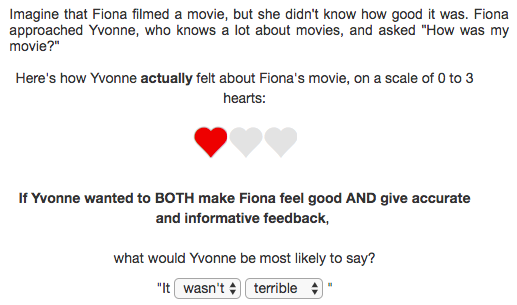
\includegraphics[width=0.7\textwidth]{fig/screenshot.png}}
%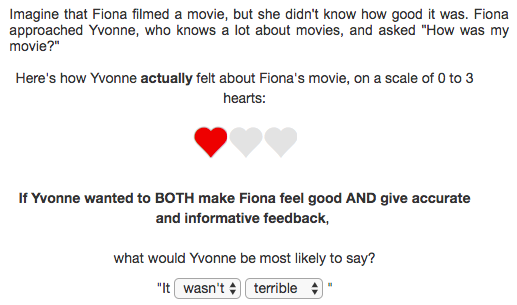
\includegraphics{fig/screenshot.png}
\caption{\label{fig:screenshot}Example of a trial in the speaker production task.}
\end{figure}

We used a simple procedure to empirically test whether our model is able to predict production of polite utterances. 
Participants read scenarios in which someone (e.g.~Ann) gave a performance of some kind, 
and another person (Bob) evaluated it. 
We provided information on Ann's feelings toward the presentation (\emph{true state}), 
which were shown on a scale from zero to three hearts 
(e.g.~one out of three hearts filled in red color; see Figure 1). 
We also presented Ann's goal, which was one of the following: 
to be \emph{informative} and give accurate feedback; 
to be \emph{social} and to make Bob feel good; 
or to be \emph{both} informative and social at the same time. 
We hypothesized that speakers with both goals to be informative and social given bad true states (i.e.~Bob's performance was poor) would produce more negation (\enquote{It wasn't\textasciitilde{}}) to save the listener's face while vaguely conveying the bad true state 
(see our pre-registered model, hypothesis, and procedure at FIXME). 
Each participant read 12 scenarios total (4 true states \(\times\) 3 goals).

In a single trial, each scenario was followed by a question that asked for the most likely utterance by Ann. 
Participants indicated their answer by choosing one of the options on the two dropdown menus, 
side-by-side, one for choosing between \emph{It was} vs. \emph{It wasn't} and the other for choosing among \emph{terrible}, \emph{bad}, \emph{good}, and \emph{amazing}, 
thereby selecting one of eight possible utterances (see Figure \ref{fig:screenshot}). 
We separately gathered the literal meaning judgments for the eight possible utterances, 
by measuring how likely each utterance is to be true given each true state, to set expected
literal meanings of utterances in our model 
(see Supplementary Materials for literal semantic results).

\begin{figure}
\centering
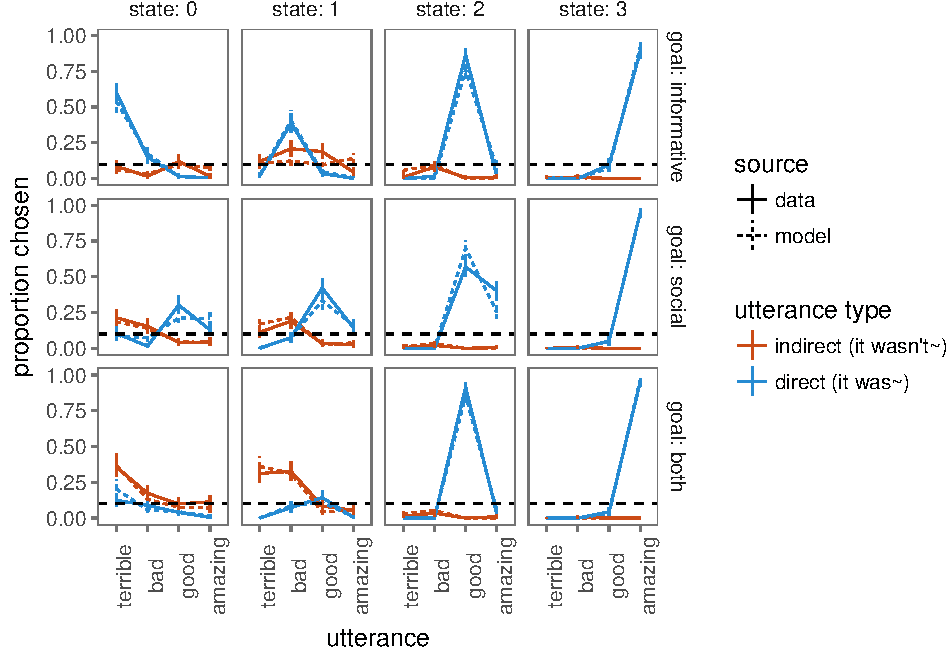
\includegraphics{politeness_files/figure-latex/utterancePrediction-1.pdf}
\caption{\label{fig:utterancePrediction}Experimental results (solid lines) and fitted model predictions (dashed lines) for speaker production.
Proportion of utterances chosen (utterance type -- direct vs.~indirect -- in different colors and words shown on x-axis) given the true states (columns) and speaker goals (rows). Error bars represent 95\% confidence intervals for the data and 95\% highest density intervals for the model.
Black dotted line represents the chance level.}
\end{figure}

\begin{figure}
\centering
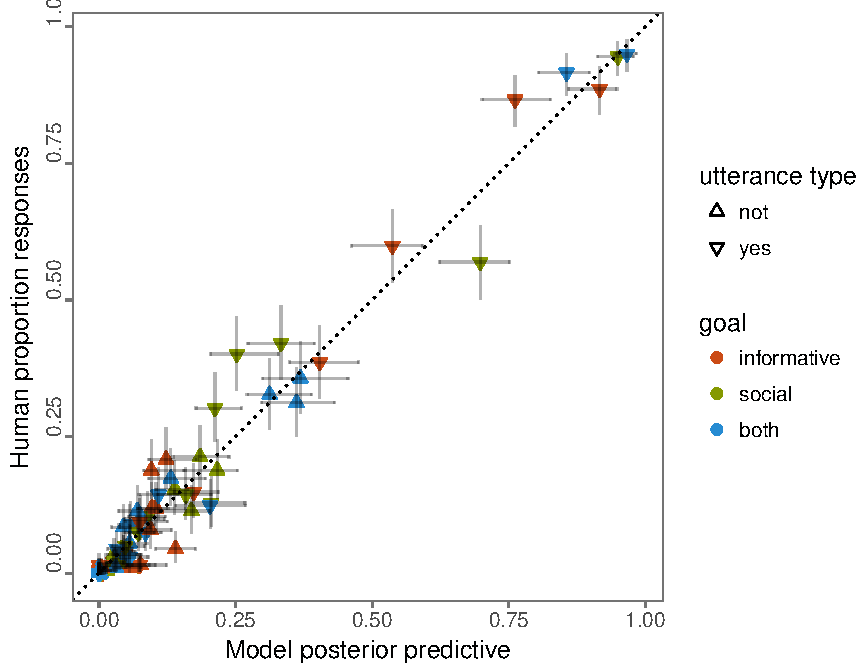
\includegraphics{politeness_files/figure-latex/varianceExplained-1.pdf}
\caption{\label{fig:varianceExplained}Full distribution of human responses vs.~model predictions. Error bars represent 95\% confidence intervals for the data (vertical) and 95\% highest density intervals for the model (horizontal).}
\end{figure}

\begin{figure}
\centering
  \makebox[\textwidth]{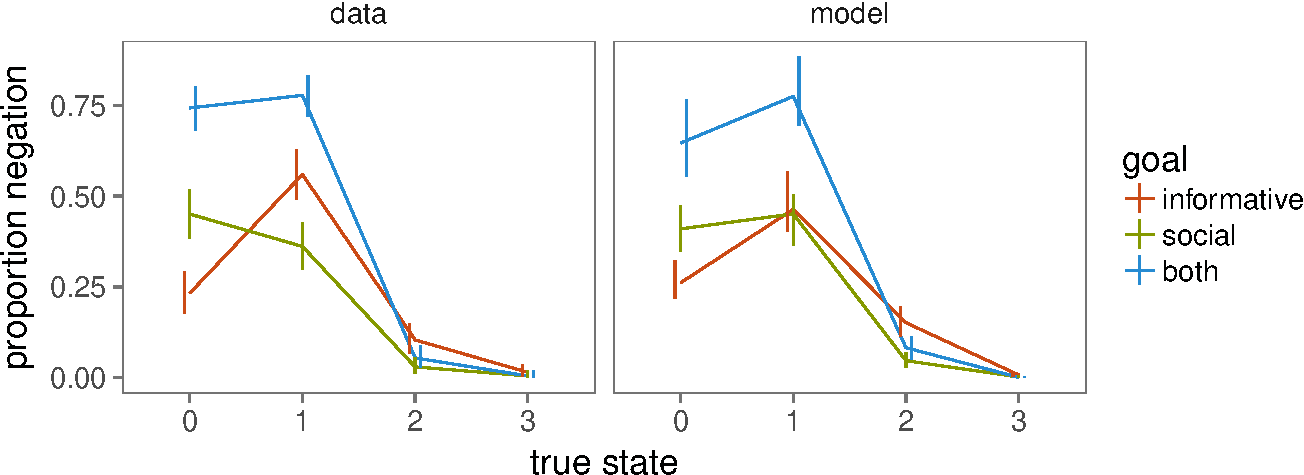
\includegraphics[width=\textwidth]{politeness_files/figure-latex/negationPrediction-1.pdf}}
%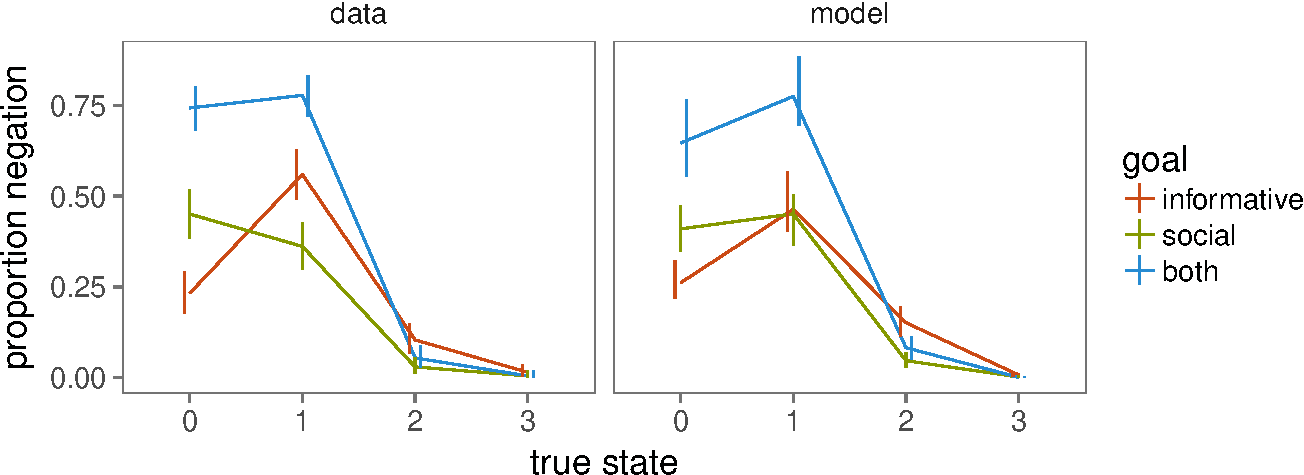
\includegraphics{politeness_files/figure-latex/negationPrediction-1.pdf}
\caption{\label{fig:negationPrediction}Experimental results (left) and fitted model predictions (right) for average proportion of negation produced among all utterances, given true states (x-axis) and goals (colors).}
\end{figure}

Mean proportion of utterances chosen by participants in each true-state \(\times\) goal condition were overall highly consistent with the our model predictions (Figure \ref{fig:utterancePrediction}). 
The posterior predictive of the model explained almost all of the variance in the production data (\(r^2\)(96) = 0.97; Figure \ref{fig:varianceExplained}). 
In line with our hypothesis, conditions in which the both-goal speaker tried to convey bad true state (0 or 1 heart) yielded the greatest proportions of negation (\enquote{It wasn't \textasciitilde{}}; see Figure \ref{fig:negationPrediction}).

Our work unifies previous formal models of communication and informal
theories of social uses of language. Our findings suggest that neither
epistemic nor social motives alone motivate polite speech; instead,
production of polite speech results from the conflict between these two,
combined with a self-presentational desire to \emph{look} epistemically
and socially helpful. These findings provide strong support for a
utility-theoretic framing of politeness, and suggest new directions in
understanding of pragmatic language use in social contexts.

% Your references go at the end of the main text, and before the
% figures.  For this document we've used BibTeX, the .bib file
% scibib.bib, and the .bst file Science.bst.  The package scicite.sty
% was included to format the reference numbers according to *Science*
% style.

%BibTeX users: After compilation, comment out the following two lines and paste in
% the generated .bbl file. 

\bibliography{politeness}

\bibliographystyle{Science}





\section*{Acknowledgments}
This work was supported by NSERC PGS Doctoral scholarship PGSD3-454094-2014 to EJY, NSF Graduate Research Fellowship DGE-114747 to MHT, ONR grant N00014-13-1-0788 to NDG, and NSF grant BCS 1456077 to MCF.

%Here you should list the contents of your Supplementary Materials -- below is an example. 
%You should include a list of Supplementary figures, Tables, and any references that appear only in the SM. 
%Note that the reference numbering continues from the main text to the SM.
% In the example below, Refs. 4-10 were cited only in the SM.     

\section*{Supplementary materials}

\subsection*{Materials and Methods}

\subsubsection*{Literal semantic task}

We probed judgments of literal meanings of the target words assumed by our model and used in all our experiments. 
51 participants with IP addresses in the United States were recruited on Amazon's Mechanical Turk. 
We used 13 different context items in which someone evaluated a performance of some kind. 
For example, in one of the contexts, Ann saw a presentation, and Ann's feelings toward the presentation (\emph{true state}) were shown on a scale from zero to three hearts 
(e.g., two out of three hearts filled in red color). 
The question of interest was "Do you think Ann thought the presentation was / wasn't X?" and participants responded by choosing either \enquote{no} or \enquote{yes.}  
The target could be one of five possible words: \emph{terrible}, \emph{bad}, \emph{good}, and \emph{amazing}, giving rise to ten different possible utterances (with negation or no negation). 
Each participant read 32 scenarios, depicting every possible combination of states and utterances. 
The order of context items was randomized, and there were a maximum of four repeats of each context item per participant. 
For this and the subsequent experiment, we analyzed the data by collapsing across context items. 

For each utterance-state pair, we computed the posterior distribution over the semantic weight 
(i.e., how consistent X utterance is with Y state) assuming a uniform prior over the weight.
Meanings of the words as judged by participants were as one would expect (see Figure \ref{fig:litSem}). 
We used the fraction of participants that endorsed utterance $w$ for state $s$ to set informative priors to infer posterior credible values of the literal meanings from data in the speaker production experiment.

\subsubsection*{Speaker production task}

202 participants with IP addresses in the United States were recruited on Amazon's Mechanical Turk.
As in the semantics measurements above, we used scenarios in which a person (e.g., Bob) gave some performance and asked for another person (e.g., Ann)'s opinion on the performance. 
Additionally, we provided information on the speaker Ann's goal -- \emph{to make Bob feel good}, or \emph{to give as accurate and informative feedback as possible}, or \emph{both} -- 
and the true state -- how Ann actually felt about Bob's performance (e.g., two out of three hearts, on a scale from zero to three hearts). 
Each participant read 12 scenarios, depicting every possible combination of goals and states. 
The order of context items was randomized, and there were a maximum of two repeats of each context item per participant.

Each scenario was followed by a question that read, "If Ann wanted \emph{to make Bob feel good} but not necessarily give informative feedback (or \emph{to give accurate and informative feedback} but not necessarily make Bob feel good, or \emph{BOTH make Bob feel good AND give accurate and informative feedback}), what would Ann be most likely to say?" Participants indicated their answer by choosing one of the options on the two dropdown menus, side-by-side, one for choosing between \emph{It was} vs. \emph{It wasn't} and the other for choosing among \emph{terrible}, \emph{bad}, \emph{good}, and \emph{amazing}.

\subsection*{Supplementary Text}

\subsubsection*{Model fitting}

We ran 4 MCMC chains for 40,000 iterations, discarding the first 20,000 for burnin. 

\subsubsection*{Inferred parameters}

In the speaker production task, participants were told what speakers' intentions were 
(e.g.~wanted to make Bob feel good). 
We assume that the intention descriptions conveyed the weight mixtures $\phi_{epistemic}$, $\phi_{social}$, $\phi_{self}$ and $\phi_{S_1}$ that the speaker was using. 
We put uninformative priors on each of these mixtures ($\phi \sim$ Uniform(0,1)) 
and inferred their credible values separately for each goal condition ("wanted to X") 
using Bayesian data analytic techniques \cite{lee2014}. 
For the \enquote{wanted to give informative feedback} (\emph{informative}) condition, FIXME. 
For the \enquote{wanted to make [listener] feel good} (\emph{social}) condition, FIXME. 
For the \enquote{wanted BOTH to make [the listener] feel good and give informative feedback} (\emph{both}) condition, FIXME (see Figure \ref{fig:goalWeights}). 

There were two additional parameters of the model, on which we put uninformative priors: the value scale parameter ($\alpha \sim $Unif(0,10)) in the utility function; and the cost parameter ($C(u) \sim $Unif(1,10)). We inferred their posterior credible values from the data. The Maximum A-Posteriori (MAP) estimates and 95\% Highest Probability Density Intervals (HDI) were: FIXME (see Figure \ref{fig:params}).

\subsubsection*{Model parameter and weight comparison}

Here we compare predictions of the current model with its possible
alternatives. The current model has a triple mixture structure, with
three goals each of which is assigned a different weight: (1) goal to be
truly informative (i.e.~want to convey the true state); (2) goal to be
truly social (i.e.~want to make the listener feel good); (3)
self-presentational goal to appear certain way (as determined by
$\phi_{S_1} $). Alternative models include one or two out of these three
components. Below we show that the current model with all three utility components
best captures the production pattern in the empirical data.

FIXME: talk about the two figures.

\subsubsection*{Data analysis tools}

We used R (3.4.2, R Core Team, 2017) and the R-packages \emph{bindrcpp}
(0.2, Müller, 2017), \emph{binom} (1.1.1, Dorai-Raj, 2014), \emph{coda}
(0.19.1, Plummer, Best, Cowles, \& Vines, 2006), \emph{dplyr} (0.7.4,
Wickham, Francois, Henry, \& Müller, 2017), \emph{forcats} (0.2.0,
Wickham, 2017a), \emph{ggplot2} (2.2.1, Wickham, 2009), \emph{ggthemes}
(3.4.0, Arnold, 2017), \emph{gridExtra} (2.3, Auguie, 2017),
\emph{jsonlite} (1.5, Ooms, 2014), \emph{langcog} (0.1.9001, Braginsky,
Yurovsky, \& Frank, n.d.), \emph{magrittr} (1.5, Bache \& Wickham,
2014), \emph{papaja} (0.1.0.9492, Aust \& Barth, 2017), \emph{purrr}
(0.2.4, Henry \& Wickham, 2017), \emph{readr} (1.1.1, Wickham, Hester,
\& Francois, 2017), \emph{rwebppl} (0.1.97, Braginsky, Tessler, \&
Hawkins, n.d.), \emph{stringr} (1.2.0, Wickham, 2017b), \emph{tibble}
(1.3.4, Müller \& Wickham, 2017), \emph{tidyr} (0.7.2, Wickham \& Henry,
2017), and \emph{tidyverse} (1.2.1, Wickham, 2017c) for all our
analyses.

%FIXME: variance explained and bayes factor

\subsection*{Figs. \ref{fig:litSem} to \ref{fig:negationPredictionComp}}

\setcounter{figure}{0}    
\beginsupplement

\begin{figure}[h]
\centering
  \makebox[\textwidth]{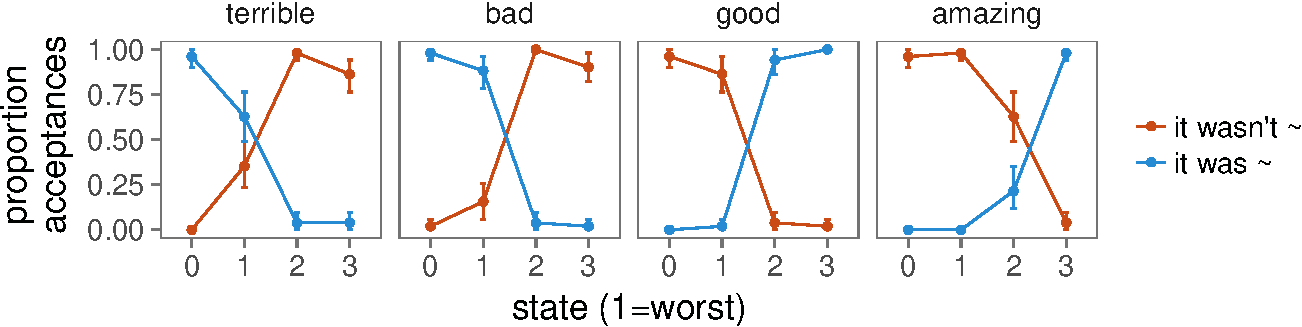
\includegraphics[width=0.8\textwidth]{politeness_files/figure-latex/litSem-1.pdf}}
\caption{\label{fig:litSem}Semantic measurement results. Proportion of
acceptances of utterance types (colors) combined with target words
(facets) given the true state represented on a scale of hearts. Error
bars represent 95\% confidence intervals.}
\end{figure}

\begin{figure}
\centering
  \makebox[\textwidth]{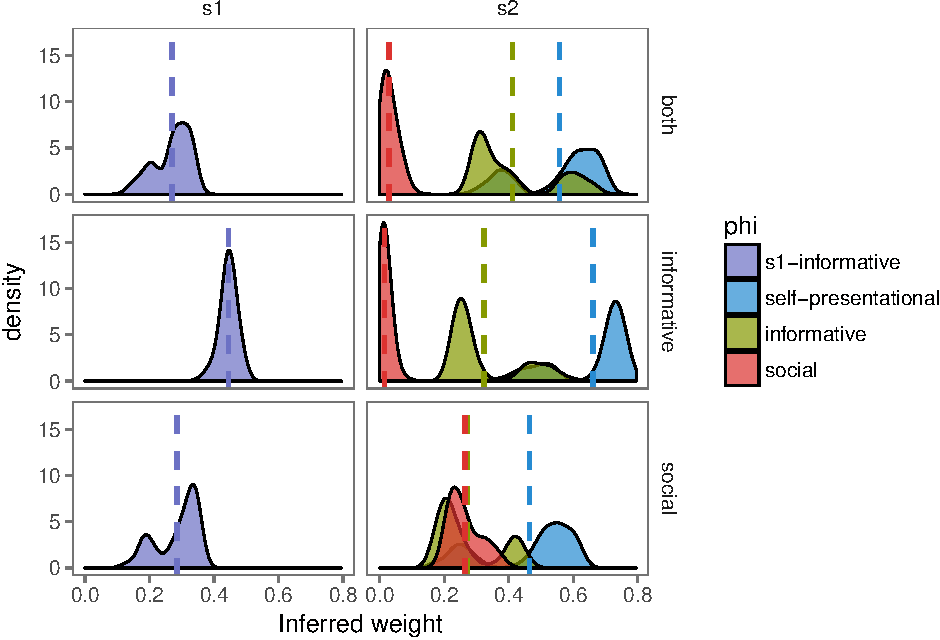
\includegraphics[width=0.9\textwidth]{politeness_files/figure-latex/goalWeights-1.pdf}}
\caption{\label{fig:goalWeights}Inferred goal weights for the main model. 
Horizontal facets are different experimental conditions (trying to be X). 
Density plots show likely weights used in the speaker's utility function.}
\end{figure}

\begin{figure}
\centering
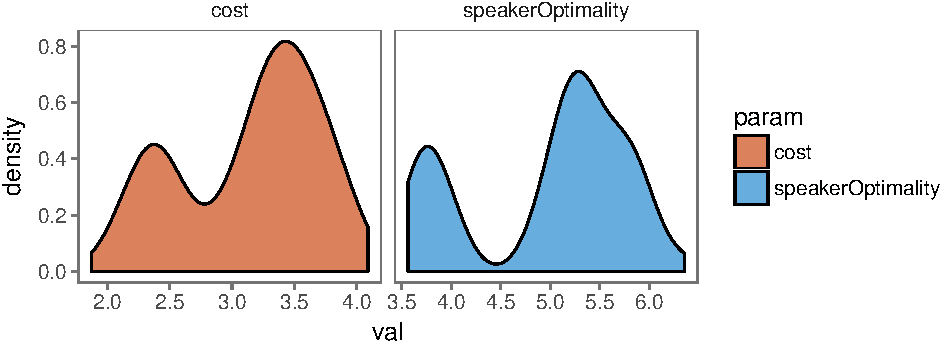
\includegraphics{politeness_files/figure-latex/params-1.pdf}
\caption{\label{fig:params}Inferred cost and speaker optimality parameters
from the main model.}
\end{figure}

\begin{figure}
\centering
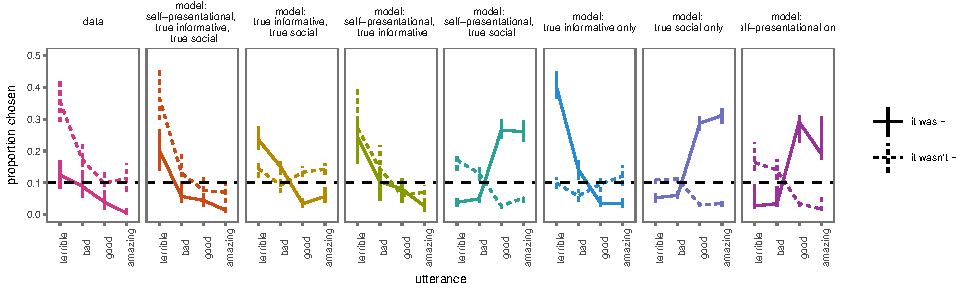
\includegraphics{politeness_files/figure-latex/utterancePredictionComp-1.pdf}
\caption{\label{fig:utterancePredictionComp}Utterances from data (leftmost)
and predictions from different model alternatives for a speaker with
both goals addressing the true state of 0 heart. Proportion of
utterances chosen (direct utterances in solid lines and indirect
utterances in dotted lines, and words shown on x-axis). Error bars
represent 95\% confidence intervals for the data and 95\% highest
density intervals for the model. Black dotted line represents the chance
level.}
\end{figure}

\begin{figure}
\centering
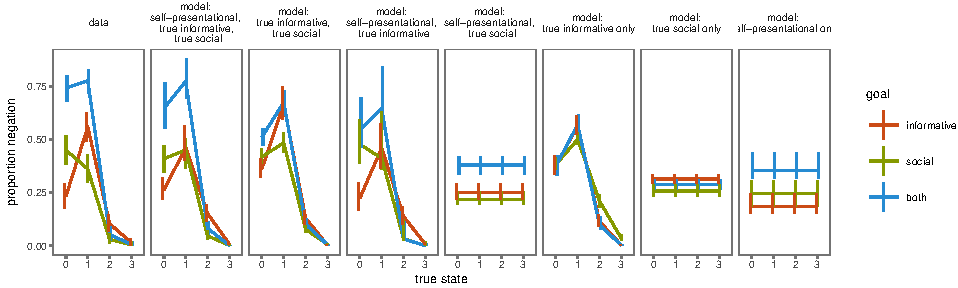
\includegraphics{politeness_files/figure-latex/negationPredictionComp-1.pdf}
\caption{\label{fig:negationPredictionComp}Experimental results (leftmost)
and predictions from different model alternatives for average proportion
of negation produced among all utterances, given true states (x-axis)
and goals (colors).}
\end{figure}

%\begin{figure}
%\centering
%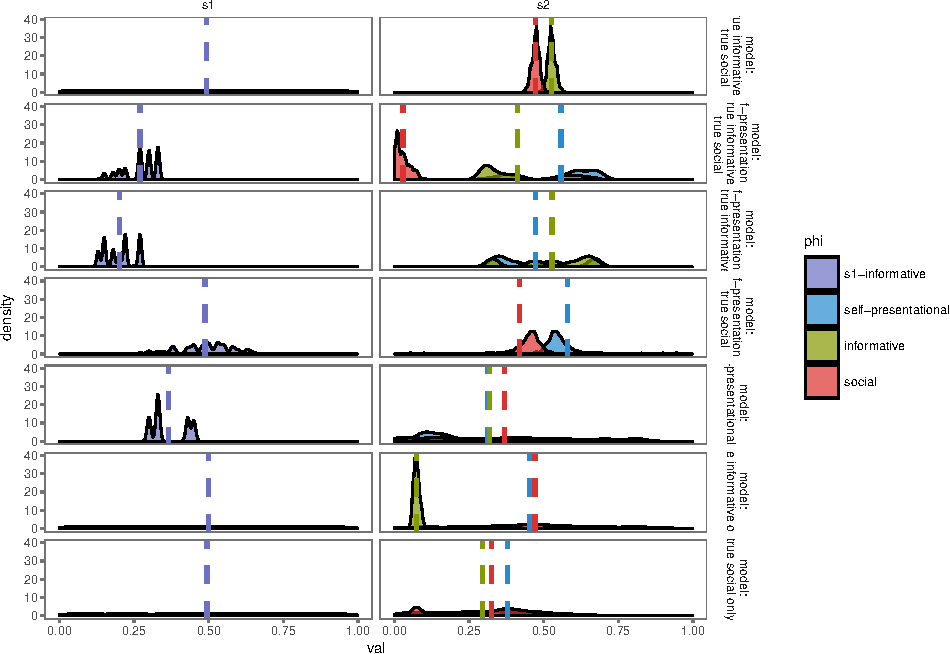
\includegraphics{politeness_files/figure-latex/goalWeightsComp-1.pdf}
%\caption{\label{fig:goalWeightsComp}Inferred goal weights from different
%model alternatives. Horizontal facets are different experimental
%conditions (trying to be X). Density plots show likely weights used in
%the speaker's utility function.}
%\end{figure}

%References \textit{(4-10)}


% For your review copy (i.e., the file you initially send in for
% evaluation), you can use the {figure} environment and the
% \includegraphics command to stream your figures into the text, placing
% all figures at the end.  For the final, revised manuscript for
% acceptance and production, however, PostScript or other graphics
% should not be streamed into your compliled file.  Instead, set
% captions as simple paragraphs (with a \noindent tag), setting them
% off from the rest of the text with a \clearpage as shown  below, and
% submit figures as separate files according to the Art Department's
% instructions.


%\clearpage
%
%\noindent {\bf Fig. 1.} Please do not use figure environments to set
%up your figures in the final (post-peer-review) draft, do not include graphics in your
%source code, and do not cite figures in the text using \LaTeX\
%\verb+\ref+ commands.  Instead, simply refer to the figure numbers in
%the text per {\it Science\/} style, and include the list of captions at
%the end of the document, coded as ordinary paragraphs as shown in the
%\texttt{scifile.tex} template file.  Your actual figure files should
%be submitted separately.

\end{document}




















